% !TEX root = ../main.tex

\section{Expression Pedal Wiring}
\label{sec:pedal-wiring}

\scaffold{
  \textbf{Paragraph 1.} Link: \cref{ch:introduction} named the two common wirings. Show them in \cref{fig:pedal-wirings} and name each panel: wiper on the tip with ring as reference and sleeve as ground, wiper on the ring with tip as reference \cite{mission2014expression, nonlinearlabs2026pedals}, and the two-wire variants that connect only tip and sleeve. Point out that the sleeve is a track end in both common three-wire wirings; \cref{sec:following} builds the position convention on this.
}

\begin{figure}[htbp]
  \centering
  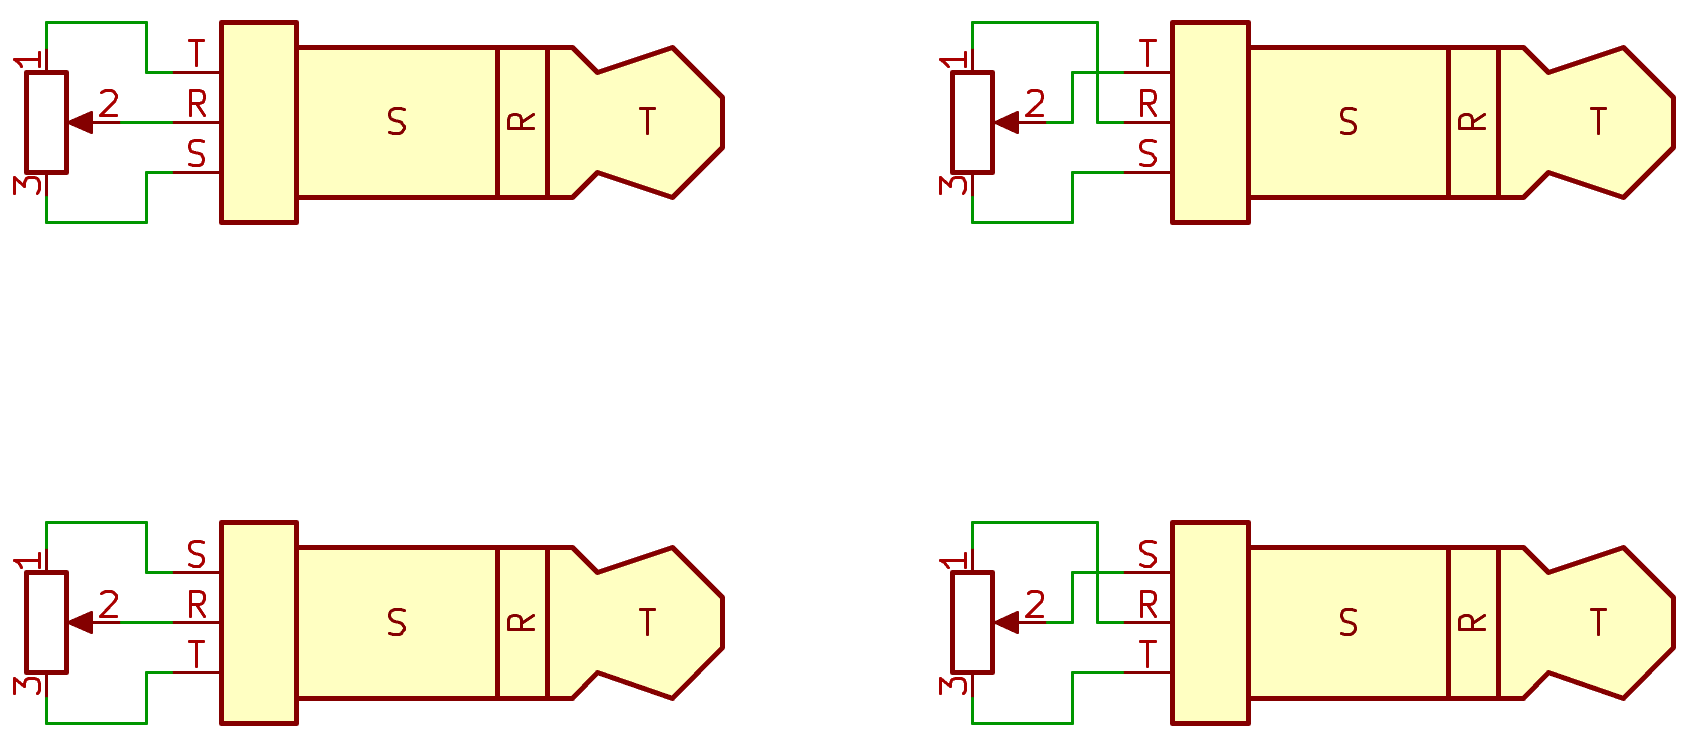
\includegraphics[width=0.85\linewidth]{03-measurement-principle/figures/pedal-wirings}
  \titledcaption{Expression Pedal Wirings}{\scaffoldinline{Name the four panels (which contact carries the wiper, which end goes to the sleeve, which variant is two-wire) and say that the potentiometer symbol is the pedal and the plug drawing the TRS plug. Source: drawing from the final presentation; check whether the four panels match the four cases named in the text, otherwise redraw.}}
  \label{fig:pedal-wirings}
\end{figure}

\scaffold{
  \textbf{Paragraph 2, pedal types and plugs.} Besides potentiometer pedals, the interface accepts sustain switches and two-wire rheostats. Which contacts conduct depends on the plug: a mono (TS) plug shorts the jack's ring contact to its sleeve, a stereo (TRS) plug leaves it unconnected. \Cref{tab:pedal-networks} lists the resulting networks; it is the reference the classification in \cref{sec:following} checks against.
}

\begin{table}[htbp]
  \centering
  \titledcaption{Pedal Networks Behind Mono and Stereo Plugs}{\scaffoldinline{Explain that each cell names which jack contacts conduct; source: \code{docs/fast-tracking.md} of the project repository.}}
  \label{tab:pedal-networks}
  \begin{tabularx}{\linewidth}{@{}l>{\raggedright\arraybackslash}X>{\raggedright\arraybackslash}X@{}}
    \toprule
    \textbf{Pedal} & \textbf{Mono plug (TS)} & \textbf{Stereo plug (TRS)} \\
    \midrule
    Potentiometer & track halves in parallel (see text) & three arms, wiper near the star point \\
    Switch, released & tip open, ring and sleeve shorted & nothing conducts \\
    Switch, pressed & all contacts shorted & tip and sleeve shorted, ring open \\
    Rheostat & tip carries it, ring and sleeve shorted & tip and sleeve carry it, ring open \\
    Cable without pedal & as a released switch & nothing conducts \\
    \bottomrule
  \end{tabularx}
\end{table}

\scaffold{
  \textbf{Paragraph 3, the mono-cable limit.} Most pedals' own jacks short their ring terminal to the sleeve when a mono plug is inserted. For a potentiometer this puts the two track halves in parallel, which gives the resistance $R\,x(1-x)$ at travel $x$ for a track of $R$: zero at both ends and $R/4$ in the middle. Derive this in one line. Conclude that the position cannot be recovered from any measurement, so potentiometer pedals need a stereo cable; this is a property of the pedal, not of the interface.
}
